\documentclass[twoside]{book}

% Packages required by doxygen
\usepackage{fixltx2e}
\usepackage{calc}
\usepackage{doxygen}
\usepackage[export]{adjustbox} % also loads graphicx
\usepackage{graphicx}
\usepackage[utf8]{inputenc}
\usepackage{makeidx}
\usepackage{multicol}
\usepackage{multirow}
\PassOptionsToPackage{warn}{textcomp}
\usepackage{textcomp}
\usepackage[nointegrals]{wasysym}
\usepackage[table]{xcolor}

% Font selection
\usepackage[T1]{fontenc}
\usepackage[scaled=.90]{helvet}
\usepackage{courier}
\usepackage{amssymb}
\usepackage{sectsty}
\renewcommand{\familydefault}{\sfdefault}
\allsectionsfont{%
  \fontseries{bc}\selectfont%
  \color{darkgray}%
}
\renewcommand{\DoxyLabelFont}{%
  \fontseries{bc}\selectfont%
  \color{darkgray}%
}
\newcommand{\+}{\discretionary{\mbox{\scriptsize$\hookleftarrow$}}{}{}}

% Page & text layout
\usepackage{geometry}
\geometry{%
  a4paper,%
  top=2.5cm,%
  bottom=2.5cm,%
  left=2.5cm,%
  right=2.5cm%
}
\tolerance=750
\hfuzz=15pt
\hbadness=750
\setlength{\emergencystretch}{15pt}
\setlength{\parindent}{0cm}
\setlength{\parskip}{3ex plus 2ex minus 2ex}
\makeatletter
\renewcommand{\paragraph}{%
  \@startsection{paragraph}{4}{0ex}{-1.0ex}{1.0ex}{%
    \normalfont\normalsize\bfseries\SS@parafont%
  }%
}
\renewcommand{\subparagraph}{%
  \@startsection{subparagraph}{5}{0ex}{-1.0ex}{1.0ex}{%
    \normalfont\normalsize\bfseries\SS@subparafont%
  }%
}
\makeatother

% Headers & footers
\usepackage{fancyhdr}
\pagestyle{fancyplain}
\fancyhead[LE]{\fancyplain{}{\bfseries\thepage}}
\fancyhead[CE]{\fancyplain{}{}}
\fancyhead[RE]{\fancyplain{}{\bfseries\leftmark}}
\fancyhead[LO]{\fancyplain{}{\bfseries\rightmark}}
\fancyhead[CO]{\fancyplain{}{}}
\fancyhead[RO]{\fancyplain{}{\bfseries\thepage}}
\fancyfoot[LE]{\fancyplain{}{}}
\fancyfoot[CE]{\fancyplain{}{}}
\fancyfoot[RE]{\fancyplain{}{\bfseries\scriptsize Generated by Doxygen }}
\fancyfoot[LO]{\fancyplain{}{\bfseries\scriptsize Generated by Doxygen }}
\fancyfoot[CO]{\fancyplain{}{}}
\fancyfoot[RO]{\fancyplain{}{}}
\renewcommand{\footrulewidth}{0.4pt}
\renewcommand{\chaptermark}[1]{%
  \markboth{#1}{}%
}
\renewcommand{\sectionmark}[1]{%
  \markright{\thesection\ #1}%
}

% Indices & bibliography
\usepackage{natbib}
\usepackage[titles]{tocloft}
\setcounter{tocdepth}{3}
\setcounter{secnumdepth}{5}
\makeindex

% Hyperlinks (required, but should be loaded last)
\usepackage{ifpdf}
\ifpdf
  \usepackage[pdftex,pagebackref=true]{hyperref}
\else
  \usepackage[ps2pdf,pagebackref=true]{hyperref}
\fi
\hypersetup{%
  colorlinks=true,%
  linkcolor=blue,%
  citecolor=blue,%
  unicode%
}

% Custom commands
\newcommand{\clearemptydoublepage}{%
  \newpage{\pagestyle{empty}\cleardoublepage}%
}

\usepackage{caption}
\captionsetup{labelsep=space,justification=centering,font={bf},singlelinecheck=off,skip=4pt,position=top}

%===== C O N T E N T S =====

\begin{document}

% Titlepage & ToC
\hypersetup{pageanchor=false,
             bookmarksnumbered=true,
             pdfencoding=unicode
            }
\pagenumbering{roman}
\begin{titlepage}
\vspace*{7cm}
\begin{center}%
{\Large Práctica 5 }\\
\vspace*{1cm}
{\large Generated by Doxygen 1.8.11}\\
\end{center}
\end{titlepage}
\clearemptydoublepage
\tableofcontents
\clearemptydoublepage
\pagenumbering{arabic}
\hypersetup{pageanchor=true}

%--- Begin generated contents ---
\chapter{Hierarchical Index}
\section{Class Hierarchy}
This inheritance list is sorted roughly, but not completely, alphabetically\+:\begin{DoxyCompactList}
\item \contentsline{section}{Client}{\pageref{class_client}}{}
\item Remote\begin{DoxyCompactList}
\item \contentsline{section}{Client\+\_\+\+Server}{\pageref{interface_client___server}}{}
\begin{DoxyCompactList}
\item \contentsline{section}{Server}{\pageref{class_server}}{}
\end{DoxyCompactList}
\end{DoxyCompactList}
\end{DoxyCompactList}

\chapter{Class Index}
\section{Class List}
Here are the classes, structs, unions and interfaces with brief descriptions\+:\begin{DoxyCompactList}
\item\contentsline{section}{{\bf main} }{\pageref{classmain}}{}
\item\contentsline{section}{{\bf Matrix} \\*\doxyref{Matrix}{p.}{class_matrix} class to create and control a integer matrix.  public }{\pageref{class_matrix}}{}
\end{DoxyCompactList}

\chapter{Class Documentation}
\hypertarget{class_client}{}\section{Client Class Reference}
\label{class_client}\index{Client@{Client}}


\hyperlink{class_client}{Client} implementation of the system  public.  


\subsection*{Static Public Member Functions}
\begin{DoxyCompactItemize}
\item 
static void \hyperlink{class_client_ac3dfeef1d2d29a91cf156064e34f1943}{plot} (int inf\+Row, int sup\+Row, int height, int width)  throws Remote\+Exception
\begin{DoxyCompactList}\small\item\em Method plot, where the client calculate the corresponding part of the image. \end{DoxyCompactList}\item 
static void \hyperlink{class_client_ab9b892ebe4b84667bfe6da7181385481}{main} (String\mbox{[}$\,$\mbox{]} args)
\begin{DoxyCompactList}\small\item\em Method Main of the project, where other programs are initialized. \end{DoxyCompactList}\end{DoxyCompactItemize}


\subsection{Detailed Description}
\hyperlink{class_client}{Client} implementation of the system  public. 

\subsection{Member Function Documentation}
\index{Client@{Client}!main@{main}}
\index{main@{main}!Client@{Client}}
\subsubsection[{\texorpdfstring{main(\+String[] args)}{main(String[] args)}}]{\setlength{\rightskip}{0pt plus 5cm}static void Client.\+main (
\begin{DoxyParamCaption}
\item[{String\mbox{[}$\,$\mbox{]}}]{args}
\end{DoxyParamCaption}
)\hspace{0.3cm}{\ttfamily [static]}}\hypertarget{class_client_ab9b892ebe4b84667bfe6da7181385481}{}\label{class_client_ab9b892ebe4b84667bfe6da7181385481}


Method Main of the project, where other programs are initialized. 


\begin{DoxyParams}{Parameters}
{\em args} & \\
\hline
\end{DoxyParams}
\begin{DoxyReturn}{Returns}
void  public static 
\end{DoxyReturn}
\index{Client@{Client}!plot@{plot}}
\index{plot@{plot}!Client@{Client}}
\subsubsection[{\texorpdfstring{plot(int inf\+Row, int sup\+Row, int height, int width)}{plot(int infRow, int supRow, int height, int width)}}]{\setlength{\rightskip}{0pt plus 5cm}static void Client.\+plot (
\begin{DoxyParamCaption}
\item[{int}]{inf\+Row, }
\item[{int}]{sup\+Row, }
\item[{int}]{height, }
\item[{int}]{width}
\end{DoxyParamCaption}
) throws Remote\+Exception\hspace{0.3cm}{\ttfamily [static]}}\hypertarget{class_client_ac3dfeef1d2d29a91cf156064e34f1943}{}\label{class_client_ac3dfeef1d2d29a91cf156064e34f1943}


Method plot, where the client calculate the corresponding part of the image. 


\begin{DoxyParams}{Parameters}
{\em integer} & inf\+Row, integer sup\+Row, integer height, integer width \\
\hline
\end{DoxyParams}
\begin{DoxyReturn}{Returns}
void 
\end{DoxyReturn}

\begin{DoxyExceptions}{Exceptions}
{\em Remote\+Exception} & public static \\
\hline
\end{DoxyExceptions}


The documentation for this class was generated from the following file\+:\begin{DoxyCompactItemize}
\item 
C\+:/\+Users/\+Alfredo/workspace/\+Practica5/src/Client.\+java\end{DoxyCompactItemize}

\hypertarget{interface_client___server}{}\section{Client\+\_\+\+Server Class Reference}
\label{interface_client___server}\index{Client\+\_\+\+Server@{Client\+\_\+\+Server}}


Is the interface of the system  public.  


Inheritance diagram for Client\+\_\+\+Server\+:\begin{figure}[H]
\begin{center}
\leavevmode
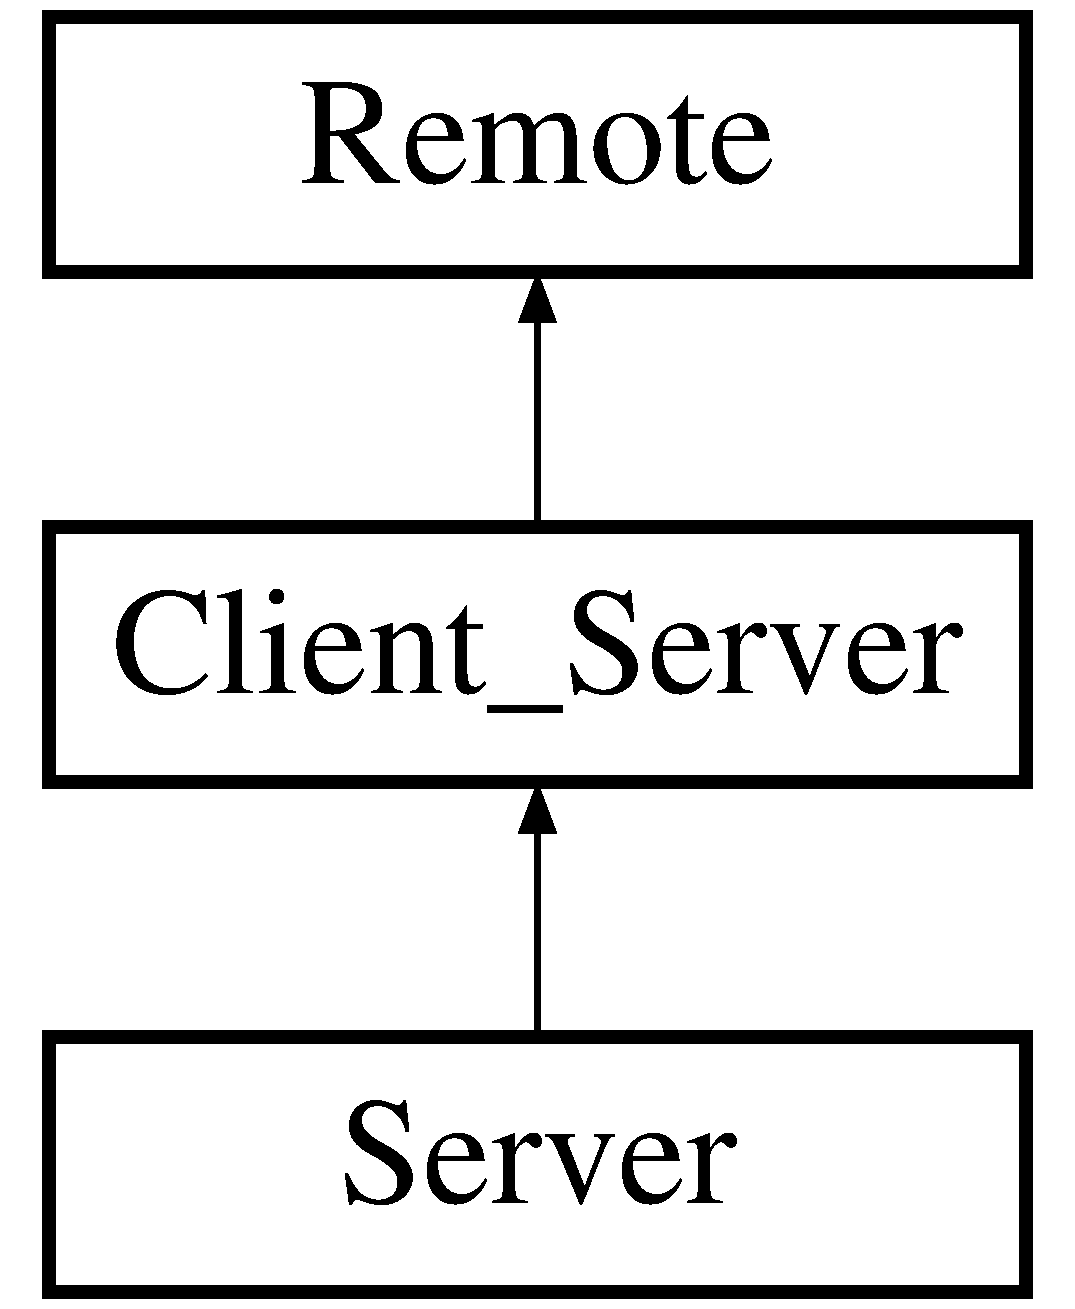
\includegraphics[height=3.000000cm]{interface_client___server}
\end{center}
\end{figure}
\subsection*{Public Member Functions}
\begin{DoxyCompactItemize}
\item 
int\mbox{[}$\,$\mbox{]} {\bfseries get\+Job} ()  throws Remote\+Exception\hypertarget{interface_client___server_ad756f998891d7bd879b6c7dd386ae78e}{}\label{interface_client___server_ad756f998891d7bd879b6c7dd386ae78e}

\item 
void {\bfseries union} (int\mbox{[}$\,$\mbox{]}\mbox{[}$\,$\mbox{]} partial\+Result, int start, int end)  throws Remote\+Exception\hypertarget{interface_client___server_ad022e27663e0ecca6418be2ca332ba7b}{}\label{interface_client___server_ad022e27663e0ecca6418be2ca332ba7b}

\end{DoxyCompactItemize}


\subsection{Detailed Description}
Is the interface of the system  public. 

The documentation for this class was generated from the following file\+:\begin{DoxyCompactItemize}
\item 
C\+:/\+Users/\+Alfredo/workspace/\+Practica5/src/Client\+\_\+\+Server.\+java\end{DoxyCompactItemize}

\hypertarget{class_server}{}\section{Server Class Reference}
\label{class_server}\index{Server@{Server}}


\hyperlink{class_server}{Server} implementation of the system  public.  


Inheritance diagram for Server\+:\begin{figure}[H]
\begin{center}
\leavevmode
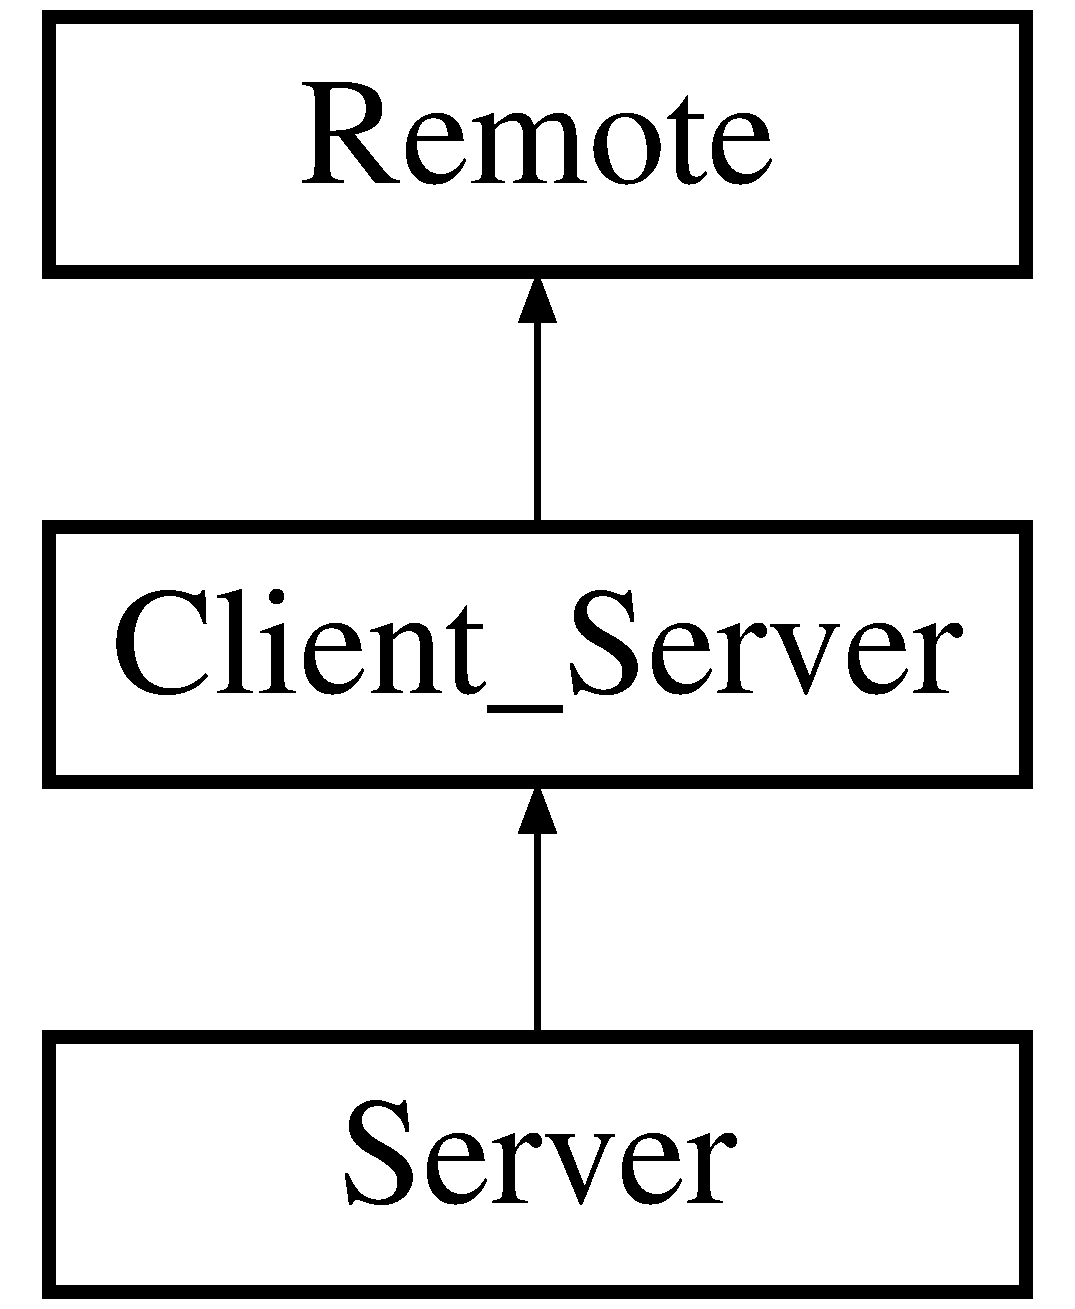
\includegraphics[height=3.000000cm]{class_server}
\end{center}
\end{figure}
\subsection*{Public Member Functions}
\begin{DoxyCompactItemize}
\item 
\hyperlink{class_server_a766ab923c89579e657e52be4f4ae2997}{Server} (int clients)
\begin{DoxyCompactList}\small\item\em \hyperlink{class_server}{Server} constructor, serves to create new clients. \end{DoxyCompactList}\item 
int\mbox{[}$\,$\mbox{]} \hyperlink{class_server_ae9a3984aeeb93c13eaccfe33612148b0}{get\+Job} ()  throws Remote\+Exception
\begin{DoxyCompactList}\small\item\em Method \hyperlink{class_server_ae9a3984aeeb93c13eaccfe33612148b0}{get\+Job()}, return jobs of the stack. \end{DoxyCompactList}\item 
void \hyperlink{class_server_ac394c6ed1551ad7ad4626ef1bbc1a2f5}{union} (int\mbox{[}$\,$\mbox{]}\mbox{[}$\,$\mbox{]} partial\+Result, int start, int end)  throws Remote\+Exception
\begin{DoxyCompactList}\small\item\em Method union, connects the parts of the result image. \end{DoxyCompactList}\end{DoxyCompactItemize}
\subsection*{Static Public Member Functions}
\begin{DoxyCompactItemize}
\item 
static void \hyperlink{class_server_ac4b46a4fdb4d54989142dee6b3e3f551}{create\+File} (String filename)  throws File\+Not\+Found\+Exception 	
\begin{DoxyCompactList}\small\item\em Method create\+File, writes in a file representation Mandelbrot. \end{DoxyCompactList}\item 
static void \hyperlink{class_server_ad90c92078da8d9c8a084e7cbc6cff4af}{main} (String args\mbox{[}$\,$\mbox{]})
\begin{DoxyCompactList}\small\item\em Method Main of the project, where other programs are initialized. \end{DoxyCompactList}\end{DoxyCompactItemize}
\subsection*{Public Attributes}
\begin{DoxyCompactItemize}
\item 
Stack$<$ int\mbox{[}$\,$\mbox{]}$>$ {\bfseries jobs}\hypertarget{class_server_ac8de6e7c3420f1bcc262d9eda19141c0}{}\label{class_server_ac8de6e7c3420f1bcc262d9eda19141c0}

\end{DoxyCompactItemize}
\subsection*{Static Public Attributes}
\begin{DoxyCompactItemize}
\item 
static int\mbox{[}$\,$\mbox{]}\mbox{[}$\,$\mbox{]} {\bfseries result}\hypertarget{class_server_a6ff98d91c732a89679431fad2c17ba4b}{}\label{class_server_a6ff98d91c732a89679431fad2c17ba4b}

\item 
static int {\bfseries Nclients}\hypertarget{class_server_aa5c8c04397758a903dda11ec51d406dc}{}\label{class_server_aa5c8c04397758a903dda11ec51d406dc}

\item 
static int {\bfseries jobsC}\hypertarget{class_server_a9cea4903754e8fe6fa8bc7d194a44f76}{}\label{class_server_a9cea4903754e8fe6fa8bc7d194a44f76}

\item 
static Registry {\bfseries registry}\hypertarget{class_server_a23960caa819012af45800c856775294a}{}\label{class_server_a23960caa819012af45800c856775294a}

\end{DoxyCompactItemize}


\subsection{Detailed Description}
\hyperlink{class_server}{Server} implementation of the system  public. 

\subsection{Constructor \& Destructor Documentation}
\index{Server@{Server}!Server@{Server}}
\index{Server@{Server}!Server@{Server}}
\subsubsection[{\texorpdfstring{Server(int clients)}{Server(int clients)}}]{\setlength{\rightskip}{0pt plus 5cm}Server.\+Server (
\begin{DoxyParamCaption}
\item[{int}]{clients}
\end{DoxyParamCaption}
)}\hypertarget{class_server_a766ab923c89579e657e52be4f4ae2997}{}\label{class_server_a766ab923c89579e657e52be4f4ae2997}


\hyperlink{class_server}{Server} constructor, serves to create new clients. 


\begin{DoxyParams}{Parameters}
{\em integer} & clients  public \\
\hline
\end{DoxyParams}


\subsection{Member Function Documentation}
\index{Server@{Server}!create\+File@{create\+File}}
\index{create\+File@{create\+File}!Server@{Server}}
\subsubsection[{\texorpdfstring{create\+File(\+String filename)}{createFile(String filename)}}]{\setlength{\rightskip}{0pt plus 5cm}static void Server.\+create\+File (
\begin{DoxyParamCaption}
\item[{String}]{filename}
\end{DoxyParamCaption}
) throws File\+Not\+Found\+Exception\hspace{0.3cm}{\ttfamily [static]}}\hypertarget{class_server_ac4b46a4fdb4d54989142dee6b3e3f551}{}\label{class_server_ac4b46a4fdb4d54989142dee6b3e3f551}


Method create\+File, writes in a file representation Mandelbrot. 


\begin{DoxyParams}{Parameters}
{\em String} & filename \\
\hline
\end{DoxyParams}
\begin{DoxyReturn}{Returns}
void 
\end{DoxyReturn}

\begin{DoxyExceptions}{Exceptions}
{\em File\+Not\+Found\+Exception} & public static \\
\hline
\end{DoxyExceptions}
\index{Server@{Server}!get\+Job@{get\+Job}}
\index{get\+Job@{get\+Job}!Server@{Server}}
\subsubsection[{\texorpdfstring{get\+Job()}{getJob()}}]{\setlength{\rightskip}{0pt plus 5cm}int \mbox{[}$\,$\mbox{]} Server.\+get\+Job (
\begin{DoxyParamCaption}
{}
\end{DoxyParamCaption}
) throws Remote\+Exception}\hypertarget{class_server_ae9a3984aeeb93c13eaccfe33612148b0}{}\label{class_server_ae9a3984aeeb93c13eaccfe33612148b0}


Method \hyperlink{class_server_ae9a3984aeeb93c13eaccfe33612148b0}{get\+Job()}, return jobs of the stack. 

\begin{DoxyReturn}{Returns}
int\mbox{[}\mbox{]}  public 
\end{DoxyReturn}
\index{Server@{Server}!main@{main}}
\index{main@{main}!Server@{Server}}
\subsubsection[{\texorpdfstring{main(\+String args[])}{main(String args[])}}]{\setlength{\rightskip}{0pt plus 5cm}static void Server.\+main (
\begin{DoxyParamCaption}
\item[{String}]{args\mbox{[}$\,$\mbox{]}}
\end{DoxyParamCaption}
)\hspace{0.3cm}{\ttfamily [static]}}\hypertarget{class_server_ad90c92078da8d9c8a084e7cbc6cff4af}{}\label{class_server_ad90c92078da8d9c8a084e7cbc6cff4af}


Method Main of the project, where other programs are initialized. 


\begin{DoxyParams}{Parameters}
{\em args} & \\
\hline
\end{DoxyParams}
\begin{DoxyReturn}{Returns}
void  public static 
\end{DoxyReturn}
\index{Server@{Server}!union@{union}}
\index{union@{union}!Server@{Server}}
\subsubsection[{\texorpdfstring{union(int[][] partial\+Result, int start, int end)}{union(int[][] partialResult, int start, int end)}}]{\setlength{\rightskip}{0pt plus 5cm}void Server.\+union (
\begin{DoxyParamCaption}
\item[{int}]{partial\+Result\mbox{[}$\,$\mbox{]}\mbox{[}$\,$\mbox{]}, }
\item[{int}]{start, }
\item[{int}]{end}
\end{DoxyParamCaption}
) throws Remote\+Exception}\hypertarget{class_server_ac394c6ed1551ad7ad4626ef1bbc1a2f5}{}\label{class_server_ac394c6ed1551ad7ad4626ef1bbc1a2f5}


Method union, connects the parts of the result image. 


\begin{DoxyParams}{Parameters}
{\em int\mbox{[}$\,$\mbox{]}\mbox{[}$\,$\mbox{]}} & partial\+Result, integer start, integer end \\
\hline
\end{DoxyParams}
\begin{DoxyReturn}{Returns}
void 
\end{DoxyReturn}

\begin{DoxyExceptions}{Exceptions}
{\em Remote\+Exception} & public \\
\hline
\end{DoxyExceptions}


The documentation for this class was generated from the following file\+:\begin{DoxyCompactItemize}
\item 
C\+:/\+Users/\+Alfredo/workspace/\+Practica5/src/Server.\+java\end{DoxyCompactItemize}

%--- End generated contents ---

% Index
\backmatter
\newpage
\phantomsection
\clearemptydoublepage
\addcontentsline{toc}{chapter}{Index}
\printindex

\end{document}
